\documentclass[a4paper]{article}

\usepackage{listings}
\usepackage{graphicx}
\begin{document}

\title{Programming the AT89S8252 using SPI}
\date{August 5, 2003}
\author{Jelmer Vernooij}
\maketitle

\begin{abstract}
    Copyright \copyright\ 2003  Jelmer Vernooij (jelmer@samba.org).
    Permission is granted to copy, distribute and/or modify this document
    under the terms of the GNU Free Documentation License, Version 1.2
    or any later version published by the Free Software Foundation;
    with no Invariant Sections, no Front-Cover Texts, and no Back-Cover Texts.
    A copy of the license is included in the section entitled ``GNU
    Free Documentation License''.
\end{abstract}

\lstset{language=C}

\tableofcontents

\section{Introduction}

The 8051 and 8052 microprocessors are very common processors. Quite some 
manufacturers (among them are Intel, Atmel and Analog Devices) produce 8051
processors. Personally, I have experience with the Atmel and the Analog Devices
processors. 

Atmel's 8051 processors can be programmed with two different protocols: 
a parallel protocol that I will not discuss here, and the SPI protocol. 

\section{Reasons for writing my own programmer}

There are several SPI programmers available for the Atmel 8051 series, however
only few of them are available for Linux, and none that I could find used 
a serial port or had a GUI.

Available programmers (and reasons not to use them):

\begin{itemize}
\item ponyprog --- has a GUI and is written in C++
\item 89prog --- uses the parallel port
\item sp89 --- uses the parallel port
\item atmel-isp --- only for windows, no source code available
\end{itemize}

And of course, figuring out the protocol with the help of a logic analyser and 
some datasheets is a lot of fun...

\section{The way other manufacturers do it}

Previously, for my work, I have written a programmer for Analog Devices
8051. Their protocol is quite a bit better since it uses the standard RS232
protocol. Something that also helps is the fact that their microcontroller 
acknowledges or (refuses) commands it gets, while with the AT89 processors, 
you just have to guess that the processor understood what you wanted.

Next to that, Analog Devices provided an example program that could be 
used to program the microcontroller of the serial port.

\section{Other data lines used by the Atmel}

Next to the lines necessary for SPI, there is another used for putting 
the processor in programmable mode:

\begin{itemize}
\item[RST] Reset. Used to put microprocessor in programmable state. Also used to restart running program (by toggling). (Connected to DTR on my board)
\end{itemize}

My own circuit board has uses an additional port that is used to confirm 
that CHK has been set.

When the RST port on the 8051 has been set, the processor listens for SPI 
input and handles incoming data.

\section{The SPI protocol}

So, what is SPI? SPI is a very simple serial data protocol. This means 
that bytes are send serially instead of parallel. SPI is a standard protocol 
that is used mainly in embedded devices. It falls in the same family as 
$I2C$ or $RS232$.

As can be read in Atmel's datasheets (document 0401 to be precise), 
the SPI protocol uses 3 lines:

\begin{itemize}
\item[MOSI] {\em (Master Out, Slave In)} Data line, in my case sitting on the TxD of my serial port
\item[MISO] {\em (Master In, Slave Out)} Data line, controlled by client. (In my case on CTS)
\item[SCK] The Clock (in my case on RTS of the serial port)
\end{itemize}

\subsection{How does SPI work?}

The SPI works with two parties: the slave and the master. The master controls 
the line. In my case the personal computer is the master and the 8051 is 
the slave. There is another data line ({\em Slave Select}) that is used to select 
who the slave is, but I didn't need to use that bit.

The master sets a bit on the {\em MOSI} and then generates a clock pulse, after 
which the next bit is set and another clock pulse is generated, etc.

\begin{figure}
\caption{Sending the bit pattern $0011 0100$ using SPI}

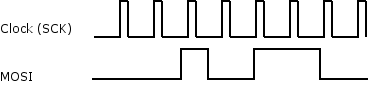
\includegraphics{SPI1}
\end{figure}

A clock pulse is generated by simply setting the {\em SCK} bit high and then low 
again after a few microseconds.

Here is my {\em SPI\_Out} function:

\begin{lstlisting}

void SPI_Out(int b)
{
	int i;
	for(i = 7; i >= 0; i--) {
		if(b & (1 << i)) SetMOSI();
		else ClearMOSI();
		waitmicrosec(2);
		SetSCK();
		waitmicrosec(3);
		ClearSCK();
		waitmicrosec(2);
	}
}

\end{lstlisting}

Reading data from the slave is done in a similar way. The server requests 
data from the slave, after which it generates clock pulses on which the slave
sets the MISO line.

My {\em SPI\_In} function:

\begin{lstlisting}
int SPI_In()
{
	int i, b = 0;
	for(i = 7; i >= 0; i--) {
		SetSCK();
		waitmicrosec(2);
		if(GetMISO())b |= 1 << i;
		waitmicrosec(3);
		ClearSCK();
		waitmicrosec(2);
	}
	return b;
}
\end{lstlisting}

That's basically all that SPI does. It's that simple!

\section{AT89* commands}

This section describes the various commands that can be sent 
to the 8051 over SPI when it's {\em RST} bit is set.

\subsection{Enabling program modus}

Before the 8051 accepts any commands, it needs to be put into command mode.
That's what this command is for. Always run this command before you 
run any other command.

\begin{lstlisting}
void programming()
{
	/* Send enable serial instruction to MOSI */
	SPI_Out(0xAC); /* 1010 1100 */
	SPI_Out(0x53); /* 0101 0011 */
	SPI_Out(0x00); /* xxxx xxxx (don't care) */
	waitmillisec(9);
}
\end{lstlisting}

\subsection{Erasing code and data memory}

\begin{lstlisting}
void erase()
{
	SPI_Out(0xAC); /* 1010 1100 */
	SPI_Out(0x04); /* xxxx x100 (x = don't care) */
	SPI_Out(0x00); /* xxxx xxxx (don't care) */
	waitmillisec(9);
}
\end{lstlisting}


\subsection{Writing data to code memory}

\begin{lstlisting}
void writecode(int addr, char b)
{
     /* hhhh h010 */
	SPI_Out(0x02 | ((addr >> 5) & 0xF8) | ((addr >> 11) & 0x04));
	SPI_Out(addr & 0xFF); /* llll llll */
	SPI_Out(b);
	waitmillisec(6);
}
\end{lstlisting}

\subsection{Reading from code memory}

\begin{lstlisting}
int readcode(int addr)
{
    /* hhhh h001 */
	SPI_Out(0x01 | ((addr >> 5) & 0xF8) | ((addr >> 11) & 0x04));
	SPI_Out(addr & 0xFF); /* llll llll */
	return SPI_In();
}
\end{lstlisting}

\subsection{Writing to data memory}

\begin{lstlisting}
void writedata(int addr, char b)
{
	SPI_Out(0x06 | ((addr >> 5) & 0xF8));
	SPI_Out(addr & 0xFF); /* llll llll */
	SPI_Out(b);
}
\end{lstlisting}

\subsection{Reading from data memory}
\begin{lstlisting}
int readdata(int addr)
{

	SPI_Out(0x05 | ((addr >> 5) & 0xF8));
	SPI_Out(addr & 0xFF); /* llll llll */
	return SPI_In();
}
\end{lstlisting}

\subsection{Locking memory}

\begin{lstlisting}
void lock(int byte)
{
	int mask = 0xff & ~byte;

	SPI_Out(0xAC);		/* 1010 1100 */
	SPI_Out(mask | 0x07);	/* pqrx x111 */
	SPI_Out(0);		/* xxxx xxxx */
	waitmillisec(9);
}
\end{lstlisting}

\section{Tips}

These are some random tips that might be useful when you are interested in
implementing the SPI protocol or the 8051 programming that is running over it.

\begin{itemize}
\item Make sure you clear and set the RST line in 
the beginning of your program
\item Make sure you wait long enough between clock pulses and that 
clock pulses are long enough
\item A logic analyser is very useful when debugging timing problems
\end{itemize}

\nocite{*}

\begin{thebibliography}{99}
\bibitem{} Atmel: AT89S8252 Datasheet, \emph{http://www.atmel.com/dyn/resources/prod\_documents/doc0401.pdf}
\bibitem{} Rob~Melby: Atmel 89 programmer, \emph{http://www.cc.gatech.edu/gvu/ccg/people/rob/software/89prog.tar.gz}
\end{thebibliography}

\end{document}
